\documentclass[review]{elsarticle}
\journal{Journal of Systems and Software}
\biboptions{authoryear,sort}

\usepackage{xspace}
\usepackage{enumitem}
\newcommand{\totalRespondents}{69\xspace}
\newcommand{\totalDevelopers}{56\xspace}
\newcommand{\totalNotDevelopers}{13\xspace}
\newcommand{\totalSearchers}{55\xspace}

\begin{document}

% -------------------------------------------------------------------------
\begin{frontmatter}

\title{Software search is not a science, even among scientists: A survey of how scientists and engineers find software}

\author[cms]{M.~Hucka}\ead{mhucka@caltech.edu}
\author[astro]{M.~J. Graham}\ead{mjg@caltech.edu}

\address[cms]{Department of Computing and Mathematical Sciences, California Institute of Technology, Pasadena, California 91125, USA}

\address[astro]{Department of Astronomy, California Institute of Technology, Pasadena, California 91125, USA}

\begin{abstract}
  If someone cannot find software for a particular task, they cannot reuse the software; thus, improved software discovery is a prerequisite for greater reuse.  However, little is known about the approaches that people use when looking for software.  We surveyed users in several technical fields to better understand their approaches and selection criteria.  We found that even in our sample of highly trained people, the relatively unsophisticated approaches of relying on general Web searches, the opinions of colleagues, and the literature were the most-often used approaches overall.  However, developers were more likely than non-developers to search in community sites such as Stack Overflow and GitHub, even when seeking ready-to-run software rather than source code.  Our results also reveal characteristics that matter to people searching for software, as well as factors that can prevent people from reusing software.
\end{abstract}

\begin{keyword}
software search \sep
software reuse \sep
software catalogs \sep
survey
\end{keyword}

\end{frontmatter}
% -------------------------------------------------------------------------


\section{Introduction}

Software is critical to research~\citep{stewart2013initial, howison2015software, howison2015understanding, ince2012case, morin_2012, hettrick_2014, hannay_2009, wilson_2006, katz2016report, katz2015looking}, yet finding software suitable for a given purpose remains surprisingly difficult~\citep{howison2015software, cannata_2005, Bourne::2015, white2014nih}.  Few resources exist to help users discover options or understand the differences between them~\citep{white2014nih}.  A recent study~\citep{bauer2014exploratory} of developers at the Internet search company Google underscored the depth of the problem: the authors found the factor ``most disruptive to the [software] reuse process'' was ``difficulties in finding artifacts.''  In other words, \emph{even developers at Google have difficulty finding software}.

Searching the Internet with a general-purpose search engine has previously been reported to be one of the most popular approaches~\citep{samadi_2004, umarji_2008}.  Despite its popularity, this approach suffers from obvious problems.  It requires thinking of appropriate search terms, which can be challenging for someone not intimately familiar with a given topic or who is not a native English speaker.  Web searches also can yield dozens of viable candidates mixed with thousands of irrelevant results, requiring the user to follow links and examine individual candidates---a time-consuming exercise.  Finally, some questions cannot be answered through Web searches without substantial additional effort, such as what are the specific characteristics of each software tool or how do tools differ from each other.  Other approaches to finding software, such as looking in the literature or asking on social media, suffer from other problems.  The difficulty of finding software and the lack of better resources brings the potential for duplication of work, reduced scientific reproducibility, and poor return on investment by funding agencies~\citep{cannata_2005, national2003sharing, crook2013learning, poisot2015best, white2014nih, niemeyer2016challenge}.

One of the first steps to providing more effective resources for finding software is to understand the factors that influence how users locate and select software today.  However, nearly all prior work on this topic has focused on developers searching for source code; most studies have ignored non-developers and/or how people look for ready-to-run software rather than source code.  In an effort to understand these other aspects, in late 2015 we conducted a survey involving members of numerous mailing lists in astronomy and systems biology.  In this article, we report on five of the research questions addressed by our survey:

\begin{description}

\item[RQ1] How do people look for ready-to-run software?
\item[RQ2] What criteria do people use to select ready-to-run software?
\item[RQ3] How do developers look for source code?
\item[RQ4] Why do developers look for source code?
\item[RQ5] What factors can prevent developers from reusing source code?

\end{description}

The remainder of this article is divided as follows. In Section~\ref{related-work}, we overview related work.  In Section~\ref{methods}, we describe our survey design and research methods, while in Section~\ref{results}, we report our results.  We discussion the results, implications and limitations in Section~\ref{discussion}, and conclude with Section~\ref{conclusions}.


\section{Related work}
\label{related-work}

Some of the our research questions have been touched on by other studies in the literature, though we could find no prior work that addressed all five questions.  We discuss relevant work in this section.


\subsection{Surveys examining how people find ready-to-run software}

Though many surveys have examined software developers and search characteristics in the context of software \emph{code} reuse, extremely few have examined how users---whether they are developers or not---go about locating \emph{ready-to-run} software.  Our research uncovered only three reports of surveys that were not focused specifically on a software development context~\citep{joppa2013troubling, huang2013provenance, lawrence2015science}.

\citet{joppa2013troubling} surveyed 596 scientists working in a single domain (biological species distribution modeling), and asked them what software they used and why they chose that particular software.  The reasons given by the respondents provide some insight into how the scientists found the software they used.  In order of most popular to least, the answers that mentioned something about ``how'' were:

\begin{itemize}[itemsep=-0.5ex]

\item ``I tried lots of software and this is the best'' (18\% of respondents)
\item ``Recommendation from close colleagues'' (18\%)
\item ``Personal recommendation'' (9\%)
\item ``Other'' (9\%)
\item ``Recommendation through a training course'' (7\%)
\item ``Because of a good presentation and/or paper I saw'' (4\%)
\item ``A reviewer suggested I use it'' (1\%)

\end{itemize}

It is worth noting that none of the responses in~\citeauthor{joppa2013troubling}'s~\citeyear{joppa2013troubling} survey explicitly mentioned searching the Internet via (e.g.)\ a Web search engine, although it is possible that some of the answers such as ``I tried lots of software and this is the best'' and ``Other'' subsumed the use of Web searches.

\citet{huang2013provenance} summarized interviews of 15 students and faculty working in bioinformatics.  They found that four factors influenced the selection of scientific software: (1) suggestions from mentors or senior members of an institution; (2) mentor involvement in the tool's development; (3) the number of publications \emph{about} the software; and (4) the software's reputation, based on the number of publications mentioning the \emph{use} of the tool.  Unfortunately, Huang et al.'s report does not include any quantitative or qualitative data about the relative importance of these factors.

\citet{lawrence2015science, lawrence2014who} conducted a large survey in 2014 about the use of science gateways by members of scientific communities.  Several of their questions and results are highly relevant to the topics of our own survey:

\begin{itemize}

% \item They asked participants to indicate domains of expertise, and permitted multiple selections.  The top five were ``Physical and Mathematical Sciences'' (30\%), ``Life Sciences'' (22\%), ``Computer and Information Sciences'' (16\%), ``Engineering'' (16\%), and ``Environmental Sciences'' (14\%), though 16\% did not indicate a domain.  Their top three fields are thus very similar to those chosen by our survey respondents (see \fig{disciplines}), though the proportions of the three are different.

\item They asked how people learn about and choose science gateways---a question related to our own survey's question about finding software (see \ref{how-find-ready-to-run}).  They found that 78\% indicated they learned about technologies from colleagues, 61\% indicated conferences and other meetings as a source, 51\% said publications, 38\% said Web searches and speciality sites, 33\% from students, and less than 10\% from mailing lists or other methods such as magazine advertisements.

% \item They asked participants about the types of Web-based resources that were important to their work from the perspective of researchers and/or educators.  The five highest rated resources where: ``Data collections'' (75\% indicated somewhat or very important), ``Data analysis tools, including visualization and mining'' (72\%), ``Computational tools'' (72\%), ``Tools for rapidly publishing and/or finding articles and data'' (69\%), and ``Educational tools'' (67\%).

\item Related to the question of how people find software, they asked software developers ``How do you keep up to date with web-based technologies?'', limiting answers to two choices from a predefined list and a free-text ``Other'' field.  The three most popular answers were: using online communities via email or Web-based forums (47\%), one's own development team (43\%), and focused workshops (18\%).

\item In another question, \citet{lawrence2015science} asked participants ``Assuming cost is not a factor, what are the most important factors you consider when adopting a new technology? Please select the three (3) most important factors in your decision-making process''.  Since this question had direct relevance to RQ2 in our survey, we include the full response results here:

\begin{itemize}[itemsep=0.2ex]
\item ``Documentation available'' (49\%)
\item ``Ability to Adapt/Customize'' (35\%)
\item ``Demonstrated Production-Quality Reliability'' (31\%)
\item ``Availability of Technical Support'' (30\%)
\item ``Open Source'' (27\%)
\item ``Existing User Community'' (20\%)
\item ``Interoperability with Other Systems'' (20\%)
\item ``Availability of Support for Bug Fixes \& Requests'' (19\%)
\item ``Testimonials/User Ratings'' (16\%)
\item ``Project Longevity'' (13\%)
\item ``Licensing Requirements'' (12\%)
\item ``Availability of Long-Term Maintenance'' (11\%)
\item ``Reputation of Those Who Built the Software'' (11\%)
\end{itemize}

\end{itemize}


\subsection{Surveys examining how developers find and reuse source code}
\label{code-search-by-developers}

Most studies of how users find software have done so in the context of software development and the reuse of software code.  In this section, we summarize the relevant studies.

\citet{samadi_2004} reported preliminary findings from a survey conducted by the NASA Earth Science Software Reuse Working Group. Their survey was distributed to government employees and contractors in the Earth science community.  Several results from the study are pertinent to our research questions:

\begin{itemize}

\item On the topic of how people found reusable software artifacts, the following approaches were noted: (1) word of mouth or personal experiences from past projects, (2) general Web search engines (e.g., Google), (3) catalogs and repositories.  The authors report ``Generic search tools (such as Google) were rated as somewhat important, whereas specialist reuse catalogs or repositories were not cited as being particularly important''.

\item As far as criteria used to decide which specific components to choose, the authors report that ``most respondents chose saving time/money and ensuring reliability as their primary drivers for reuse''.  Further, the following additional considerations were noted: (1) ``ease of adaption/integration'', (2) availability of source code'', (3) ``cost of creating/acquiring alternative'', and (4) ``recommendation from a colleague''.  The authors further report that (a) availability of support, (b) standards compliance, and (c) testing/certification, were ``not ranked as particularly important''.

\item On the topic of barriers to reuse, two common types of barriers emerged: (1) if available software did not meet a person's specific requirements, and (2) if a given software artifact was ``difficult to understand or poorly documented''.

\end{itemize}

The study was reprised in 2005 with a wider audience that included members of academia.  According to \citet{marshall2006software}, the larger 2005 survey produced essentially similar results to the preliminary 2004 survey.  They noted:

\begin{itemize}

\item The primary reason given by people for not reusing software from outside of their group was that ``they did not know where to look for reusable artifacts and they did not know suitable artifacts existed at the time.''

\item For those who did engage in reuse, ``personal knowledge from past projects and word-of-mouth or networking were the primary ways of locating and acquiring software development artifacts.''  

\item On the topic of how people located software, the results reported by \citet{marshall2006software} seem to be inconsistent.  The authors noted that ``Web searches were of average importance while serendipity and reuse catalogs or repositories were rated the lowest''; however, in another section of the survey dealing with how to increase reuse within the Earth science community, one of the top three factors was ``having an Earth science catalog/repository for reusable artifacts.''  In other words, catalogs were rated low in one part of the survey but high in another part.  Despite this, among their conclusions, Marshall et al. noted ``the use of reuse catalogs and repositories was rated the most important method of increasing the level of reuse within the community.''

\end{itemize}

In a different NASA study, Orrego and Mundy~\citep{orrego_2007_study} examined software reuse in the context of flight control systems.  They studied 63 projects using interviews, surveys and case studies.  In interviews with 15 people, they found that black-box reuse and other types of reuse did occur, and the degree to which a given project reused software ranged from 0\% to 80\%.  The difficulty of assessing the characteristics of software was stated as the most problematic aspect of reusing software, usually because of inadequate documentation for the software to be reused.

\citet{umarji_2008} \citep[also discussed in ref.][]{umarji_2013} surveyed Java programmers in 2006--2007 to understand how and why they searched for source code.  Using invitations to mailing lists and newsgroups, they solicited participation to fill out a Web survey, and received 69 responses.  Several facets of the Umarji et al.\ study are especially relevant to our own survey:

\begin{itemize}

\item With respect to developers' motivations, out of a total of~51 searches described, \citeauthor{umarji_2008} found that the largest fraction concerned finding either (a) reusable code (67\% of the 51 results), (b) reference examples (33\%), or debugging activities (10\%).  Within the first category,  \citeauthor{umarji_2008}\ identified four common search objectives: developers searched for (1) code fragments; (2) subsystems that implemented reusable data structures, algorithms, or other elements; (3) packages or API libraries; and (4) stand-alone tools or systems (in one participant's words, ``big piece of code that does more or less what I want'').  Within the category of reference examples (b), \citeauthor{umarji_2008} also identified four (different) common search goals: finding (1)  code fragments that illustrate syntax; (2) implementations of data structure, algorithm or widgets in order to verify a programmer's own approach or use as a basis for reimplementation; (3) examples of how to use a library; and (4) similar software to generate new ideas.  Within the category of debugging (c), developers searched for solutions to software defects or explanations for the cause of an error.

\item \citet{umarji_2013} report that common starting points for searches were: (1) recommendations from friends, and (2) reviews, articles, blogs and social tagging sites.

\item With respect to how developers conducted searches, the participants in the survey used the following, in order of popularity: (1) general-purpose search engines (87\% of participants), (2) personal domain knowledge (54\%), (3) project hosting sites such as SourceForge.net~\citep{sourceforge_1999} (49\%), (4) references from peers (43\%), (4) mailing lists (23\%), and (5) code-specific search engines such as Google Code Search~\citep{googlecodesearch_2006} (16\%).

\item With respect to the selection criteria used by developers to choose a solution, \citet{umarji_2013} report that the most important factors were: (1) software functionality (78\%), (2) type of software license (43\%), (3) price (38\%), (4) amount of user support available (30\%), and (5) level of project activity (26\%).

\end{itemize}

\citet{gallardo2011kinds} examined the Web search behaviors of 25 developers working at a software company that develops transactional software for banks and other organizations.  They found that 8\% of the Web searches performed by developers during the study period were to download libraries or other tools, and another 5\% of the Web searches were to collect information to help judge the suitability of software components to be used in implementations.

\citet{sim2012software} performed a pair of surveys as part of an effort to understand developers' approaches to code search.  For purposes of the current review, the quantitative survey results are more relevant.  On the topic of what subjects searched for, 92\% of respondents in their survey answered they had searched for code snippets on past occasions, and 69\% said they had searched for software components.  In terms of motivations for why they conducted searches, 96\% of participants said they had sought reference examples on past occasions, and 35\% said that they had searched for code to reuse as-is.

\citet{singer2014software} examined how software developers active on GitHub use Twitter.  They conducted an initial exploratory survey with 271 GitHub users (270 of whom said they develop software) and followed it up with a validation survey involving 1,413 GitHub users (1,412 of whom said they develop software).  Their results have the following relevance to the topic of how people find and choose software.  Developers extend their knowledge of software (including new software tools and components) by asking and answering questions, participating in conversations, and following experts.  This can lead to serendipitous discovery of reusable methods, software components and software tools.  Singer et al.\ noted ``Some developers mentioned that Twitter helps them find and learn about things that they would not have been able to search for themselves, such as emerging technologies that are too new to appear in web searches.''

\citet{bauer2014exploratory} studied reuse practices by developers at Google.  Several questions in Bauer et al.'s survey are relevant to the present study:

\begin{itemize}

\item They asked subjects for their top three ways of sharing software components.  They received 63 responses: common repository (97\%), packaged libraries (34\%), tutorials (31\%), blogs (19\%), email (9\%), ``I do not share artifacts'' (3\%), and ``other'' (3\%).

\item Bauer et al.\ asked about the preferred ways to find reusable software.  They received 106 responses: code search (77\%), communication with colleagues (64\%), Web search (49\%), browsing repositories (41\%), browsing documentation (23\%), ``other'' (8\%), ``code completion'' (5\%), code recommendation systems (3\%), and tutorials (3\%).  It is worth noting that Google has a centralized code repository where most of the code is available for all projects; this repository system features a centralized code search facility.

\item They also asked ``What do you do to properly understand and adequately select reusable artifacts?'' and received 115 responses: interface documentation (72\%), examples of usage on blogs and tutorials (64\%), reviewing implementations (64\%), reading guidelines (51\%), exploring third-party products (28\%), ``other'' (10\%), and participating in training for third-party products (5\%).

\end{itemize}

\citet{sadowski2015developers} surveyed and analyzed search behaviors of 40 software developers at Google, Inc.  They developed a Web browser extension that directed developers to a survey system whenever the developers accessed an internal code search system at the company, and asked the survey participants to install this browser extension when they worked.  The survey system asked developers four multiple-choice questions before they started a search.  Two of their survey questions are directly related to questions we also asked in our own survey.  One concerned why developers searched and what questions they tried to answer with their code search.  The most common theme (33.5\% of the survey responses) dealt with getting specific information about an API library or examples of its use.  A second question investigated by Sadowski et al.\ is the context in which code search is used.  The most common situation (39\% of survey responses) was performing searches while working on a code change during development.  In this context, almost half of the developers (46\%) used code search to understand how code worked.


\subsection{Other studies}

In addition to the related surveys reported here, there are other works not reviewed here that have applied other methods to examining developer behavior.  The two main classes of non-survey techniques have been the analysis of search engine logs~\citep{bajrachary_2009, bajracharya2012analyzing, jansen_2006, teevan_2004, brandt2009two, brandt2010example, Li2009751, ge2014developers, volske2015users}, and observational studies (often coupled with interviews), either in institutional settings or in laboratory environments~\citep{sim_2011, brandt2009two, banker1993repository, gallardo2013software, sherif2003barriers, pohthong2001reuse, sim2013controlled, murphyhill2015how, sim2011getting, dabbish_2012}.  Due to the different techniques and intentions behind these efforts, the results are outside the scope of what we can compare directly to our survey.


\section{Survey design and methods}
\label{methods}

Our survey was designed to shed light on current practices and experiences in searching for software in two different situations: looking for ready-to-run software, and looking for software source code.  Respondents did not have to be software developers themselves (although the results show that most were).  We chose to use a Web-based survey because it is an approach that (1) is well-suited to gathering information quickly from a wide audience, (2) requires modest development effort, and (3) can produce data that can be analyzed qualitatively and quantitatively.


\subsection{Instrument development}

We developed the survey instrument iteratively.  We began with an initial version in which we posed many questions related to searching for software.  Following the practices of other surveys in computing~\citep[e.g.,][]{varnellsarjeant2015comparing, kitchenham_2008}, we designed the instrument iteratively and payed attention to the following points:

\begin{itemize}

\item Wording.  We sought to make the questions clear and unambiguous, and avoid implying a particular perspective.  We elaborated each question with explanatory text under the question itself.

\item Relevance to user's experiences.  We limited our questions to topics that could reasonably be assumed to be within the experiences of our audience.

\item Contemporary circumstances.  We tried to ground the questions by referring to real resources and specific software characteristics that we believe are relevant to computer users today.

\item Ethics.  We avoided questions that might be construed as being too personal or about proprietary policies at participants' place of work.

\end{itemize}

To help iterate on the design of the survey instrument, we performed a pilot survey with a dozen colleagues as subjects.  Based on their feedback, we removed or expanded questions as necessary to achieve the final version.  The final survey form is presented in Appendix~A.  The instrument contained a total of 22 questions (of which 18 were content questions), and included conditional branches so that the final number of questions actually seen by any given respondent depended on the answers selected to certain screening questions.  There were five main groups of questions in the survey:

\begin{enumerate}

\item Basic demographic and general information, suitable for all respondents.

\item Questions for software users who have the freedom to choose software.  This section was only shown if participants indicated that they have some choice in the software they use.

\item Questions for software developers.  This section was only shown if respondents indicated that are engaged in software development.

\item Questions for software developers who search for source code.  This was only shown if respondents indicated both that they are software developers and that they search for software source code.

\item Survey feedback.  This section sought feedback about the survey itself.

\end{enumerate}

Questions in section No.~2 of the survey aimed to establish the relative importance of different search criteria.  Those in section Nos.~3 and~4 sought to characterize the experiences of the developer.

The survey form used a mixture of four types of questions: check boxes, pull-down selection menus, two-dimensional rating grids, and short-answer input fields.  Some of the questions allowed answers on a nominal scale (for example, approaches used for finding software), some questions used an ordinal scale (for example, the importance of different considerations when looking for software), and some were open-ended questions asking for free-form text.


\subsection{Administration}

We used Google Forms~\citep{googleforms} to implement the survey instrument.  The version of Google Forms was the free edition made available as of September, 2015.  We obtained prior approval for the survey protocol from the California Institute of Technology's Committee for the Protection of Human Subjects.  The survey form itself included a Web link to a copy of the informed consent form for survey participation.  The first question in the survey provided a clickable checkbox by which subjects had to indicate they had read the informed consent form and consented to our use of their responses to the survey.  This was the only question in the survey that required a response; all other responses were optional.

We generated a URL (Uniform Resource Locator) for the survey form using Google Shortener~\citep{googl}, a service that produces shortened URLs and simultaneously provides an analytics facility tied to the URL.  On September 1, 2015, we invited participation in the survey.  As mentioned below, we advertised the survey on mailing lists and social media oriented to the astronomical and biological sciences, particularly to computational subcommunities within those domains.  Recipients were free to participate if they chose.  The introduction and instructions for the survey were brief.  Sample invitation letters are included in Appendix~B.  The survey had no express closing date.


\subsection{Sampling plan}
\label{sampling-plan}

% Where we sent it:
%   cds-all: 77
%   sbml-interoperability: 62
%   sysbio: 213 (215 total - 2 disabled addresses)
%   sbml team: 6
%   facebook astronomy group (closed list): 1487
%   ivoa mailing list: 453
%
% Total: 2298

\newcommand{\totalPotentialRecipients}{2300\xspace}
\newcommand{\totalClicks}{172\xspace}
\newcommand{\accessRate}{7.5\%\xspace}
\newcommand{\populationResponseRate}{3\%\xspace}
\newcommand{\completionRate}{40\%\xspace}

We used nonprobabilistic convenience sampling with self-selection.  We advertised the survey on electronic mailing lists oriented to the astronomical and biological sciences: the \emph{IVOA} mailing list (astronomy), a Facebook astronomy list, the mailing list \texttt{sysbio@caltech.edu} (systems biology), the forum \texttt{sbml-interoperability@googlegroups.com} (systems biology), the list \texttt{cds-all@caltech.edu} (departmental list), and our immediate work colleagues (totalling a dozen people).  Taken together, the members are a mix of staff, students, and faculty working in academia, government laboratories, and industry.

Potential biasing factors in the results include those that are common to self-selected written surveys with convenience sampling: response bias (i.e., people who responded may have different characteristics than those who did not), coverage errors (i.e., the representation of participants may not be balanced across different subcommunities), and item bias (i.e., some questions may have been skipped intentionally or unintentionally).  An additional possible source of bias is that the authors are relatively well-known within the subcommunities to which the survey was advertised, which may have influenced respondents.  


\subsection{Population sample}
\label{population-sample}

We analyzed the results obtained by December 31, 2015.  We estimate the number of potential recipients of the mail announcements to be at least \totalPotentialRecipients.  The number of completed survey forms was \totalRespondents.  As mentioned above, our survey URL was backed by an analytics facility; this provided the number of URL clicks, the referrer sources, and source geographical locations.  According to this facility, the survey form was accessed \totalClicks times.  Using these three numbers, we can calculate the following:

\begin{enumerate}[itemsep=-0.5ex]

\item \emph{Estimated access rate to survey form}: approximately \accessRate  (\totalClicks/\totalPotentialRecipients).

\item \emph{Estimated response rate}: approximately \populationResponseRate (\totalRespondents/\totalPotentialRecipients).

\end{enumerate}

Unfortunately, we cannot be certain of the actual number of recipients.  While we can determine the number of addresses we contacted, some of the addresses on mailing lists may be obsolete or unreachable, or the recipients' electronic mail systems may have filtered out the mail messages.  Thus, we can only estimate the response rate.  We revisit this topic in \ref{conclusion}.


\subsection{Analysis}

Descriptive statistics were performed using custom programs written in the language Python~\citep{vanRossum1991interactively, perez2011python}, version~3.4, in combination with the NumPy~\citep{vanderwalt2011numpy} package, version~1.10.4.  The figures in this paper were generated with the help of the Python library Matplotlib~\citep{hunter2007matplotlib}, version~1.5.1.



%%%







\section{Results}
\label{results}


\subsection{Criteria used when looking for software}

The last outcome summarized above from Lawrence et al.'s survey~\citep{lawrence2015science} is surprisingly different from the results of a similar question in our survey.  Comparing the results above to our \ref{criteria-ready-to-run}, neither the relative ordering of the chosen criteria, nor the absolute positions, are consistent between the two sets of survey responses.  The differences are puzzling.  While it is true that our survey included many more possible criteria, and in addition, some criteria in Lawrence et al.'s survey question were coarser in detail, many items in both surveys are comparable, so these two differences alone are unlikely to explain the results.  It is possible that the rankings are influenced by the different answer formats: we asked participants to rank the importance of each criterion, while Lawrence et al.\ asked respondents pick their top three criteria.  In an effort to assess whether this is a possible cause, we reanalyzed our results by ranking the responses based on the sum of the number of times ``Essential'', ``Usually of above-average importance'', and ``Average importance'' were selected for each criterion.  The results are shown in \ref{criteria-ready-to-run-reranked}.  Now the quality of documentation is sixth highest in rank, and quality of the software is fourth highest, which begins to approach the high ranks these two criteria had in Lawrence et al.'s survey.  However, other features remain quite different in rankings between the survey results.

\begin{figure}[t]
  \vspace*{1ex}
  \centering
  \hspace*{-1ex}%
  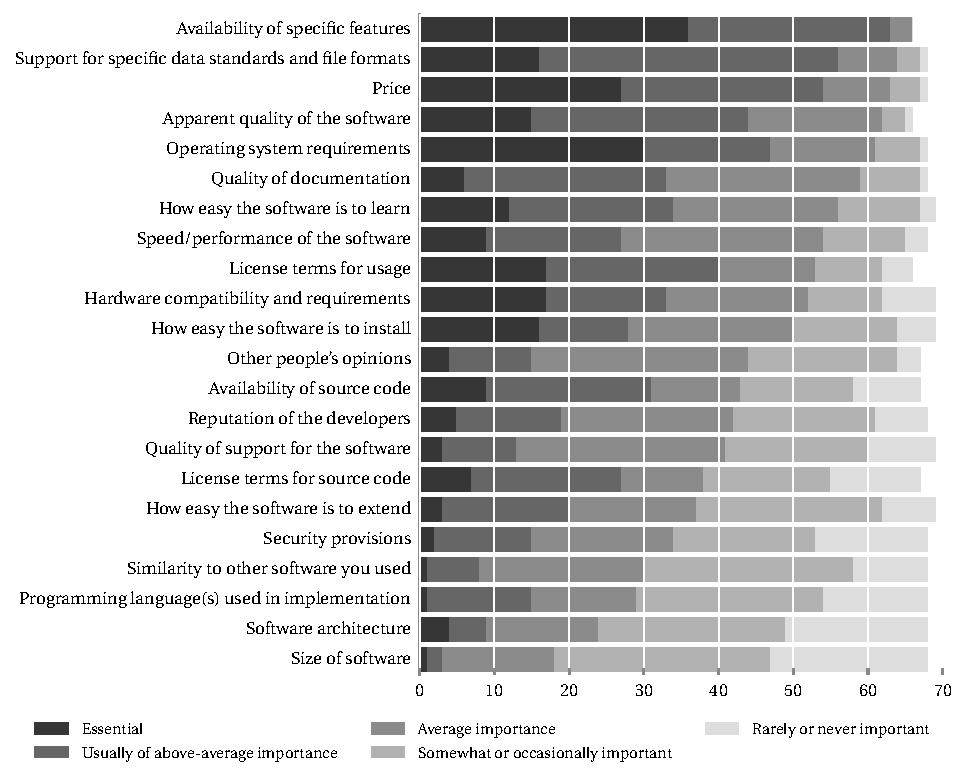
\includegraphics{files/plots/bar-graph-criteria-ready-to-run-reranked.pdf}
  \vspace*{-4ex}
  \caption{Reanalysis of the responses to the question of \protect\fig{criteria-ready-to-run}.  In this bar graph, we sorted the possible criteria by the sum of the number of times the options ``Essential'', ``Usually of above-average importance'' and ``Average importance'' were selected for each one.}
  \label{criteria-ready-to-run-reranked}
\end{figure}

Other factors therefore must be responsible for the differences in results between our survey and that of Lawrence et al.~\citep{lawrence2015science}.  We hypothesize two possibilities.  First, the context of their survey was scientific computing gateways, whereas our survey was not focused on this and considered people working with any kind of software environment.  This may influence the criteria people use to select between software options.  Second, Lawrence et al.'s survey had far more respondents than we did.  It is possible that our results for this question would be different if we had a larger sample.


\subsection{What can prevent peole}


The last result above from \citet{samadi_2004} matches the results of our survey.  For our question about what factors hindered people from finding software (\ref{reasons-for-search-failure}), the most popular reason was finding a match to one's needs, and for our question about what hindered people's ability to reuse source code found (\ref{reuse-failures}), quality of documentation was the most popular reason.




\section{Discussion}
\label{discussion}


\section{Conclusions}
\label{conclusions}


When asked, many people say they look for software by searching the Web with a general-purpose search engine~\citep{samadi_2004, umarji_2008}.  Despite its popularity, this approach suffers from significant problems: Web searches can yield dozens of viable candidates---and millions of irrelevant results.  Moreover, some questions cannot be answered through Web searches without substantial additional effort, such as what are the \emph{specific} characteristics of each software tool or how do tools \emph{differ} from each other.  Many researchers also look in the scientific literature to learn what others have used for similar tasks~\citep{lawrence2015science, joppa2013troubling}.  Searching the literature can produce more relevant results and provide other information, but it suffers from limitations too: publications are static documents that may not reflect a tool's current capabilities~\citep{wren_2004}, and moreover, not all publications describe the software they use~\citep{howison2015software}.  Still other methods for finding software include asking colleagues, asking on social media, searching scientific computing gateways, and more.  None of these 


\section{Acknowledgments}

This work was funded by the USA National Science Foundation, award \#1533792.  We thank
Daniel S. Katz,
Sarah M. Keating,
Rajiv Ramnath,
Renee M. Rottner,
Lucian P. Smith, and
Linda J. Taddeo
for many comments and feedback on previous versions of this manuscript.


\bibliographystyle{elsarticle-harv}
\bibliography{casics-survey.bib}

\end{document}
